% ==============================================================================
%                                    DVG303
%                  Objektorienterad design och programmering
%                                Laboration #2
%
% Author:   Jonas Sjöberg
%           Högskolan i Gävle
%           tel12jsg@student.hig.se
%           https://github.com/jonasjberg
%
% License:  Creative Commons Attribution-NonCommercial-ShareAlike 4.0
%           International.  See LICENSE.md for full licensing information.
% ==============================================================================

\section{Uppgift 3}\label{sec:uppg3}

\subsection{}\label{sec:uppg3a}
\subsubsection*{Frågeställning}
När metoden \texttt{createPoint} anropas på ett objekt av typen
\texttt{FigureHandler}, så måste det skickas ett antal meddelanden mellan olika
objekt. Visa meddelanden med hjälp av ett sekvensdiagram!

\subsubsection*{Lösning}
Programmet analyserades med \texttt{JIVE} -- Java Interactive
Visualization Environment. \footnote{\url{http://www.cse.buffalo.edu/jive/}}

\texttt{JIVE} installeras som en plugin i \texttt{Eclipse Mars} version 4.5.0
och körs i ett interaktivt debug-``perspective''. Programmet kan generera olika
modeller av ett exekverande program;

\begin{enumerate}
\item Contour Model.
\item Object Diagram.
\item Sequence Model.
\item Sequence Diagram.
\item Event Log.
\end{enumerate}

En särskild klass vid namn \texttt{FigureHandlerTest} användes vid körning av
\texttt{JIVE}, som presenterar resultatet på olika sätt. Jag valde att
exportera som \texttt{csv}-textfil samt \texttt{png}-bild.

Sekvensdiagram för programmet \texttt{FigureHandlerTest} återfinns i
Figur~\ref{fig:sekv-point}, Figur~\ref{fig:sekv-line},
Figur~\ref{fig:sekv-rect} och Figur~\ref{fig:sekv-all}.
Resultatet av testerna är finns också bifogade i katalogen \texttt{diagram}.

% JIVE: Dynamic Analysis for Java
% Overview, Architecture, and Implementation
% Demian Lessa
% Computer Science and Engineering
% State University of New York, Buffalo
% http://www.cse.buffalo.edu/jive/presentations/cse505-10-12-01.pdf

% Jive
% Tool Overview
% April 07 :: Spring 2010
% Demian Lessa <dlessa@buffalo.edu>
% http://www.cse.buffalo.edu/jive/presentations/cse605-10-04-07a.pdf

%\begin{sidewaysfigure}[ht]
\begin{figure}[ht]
\centering
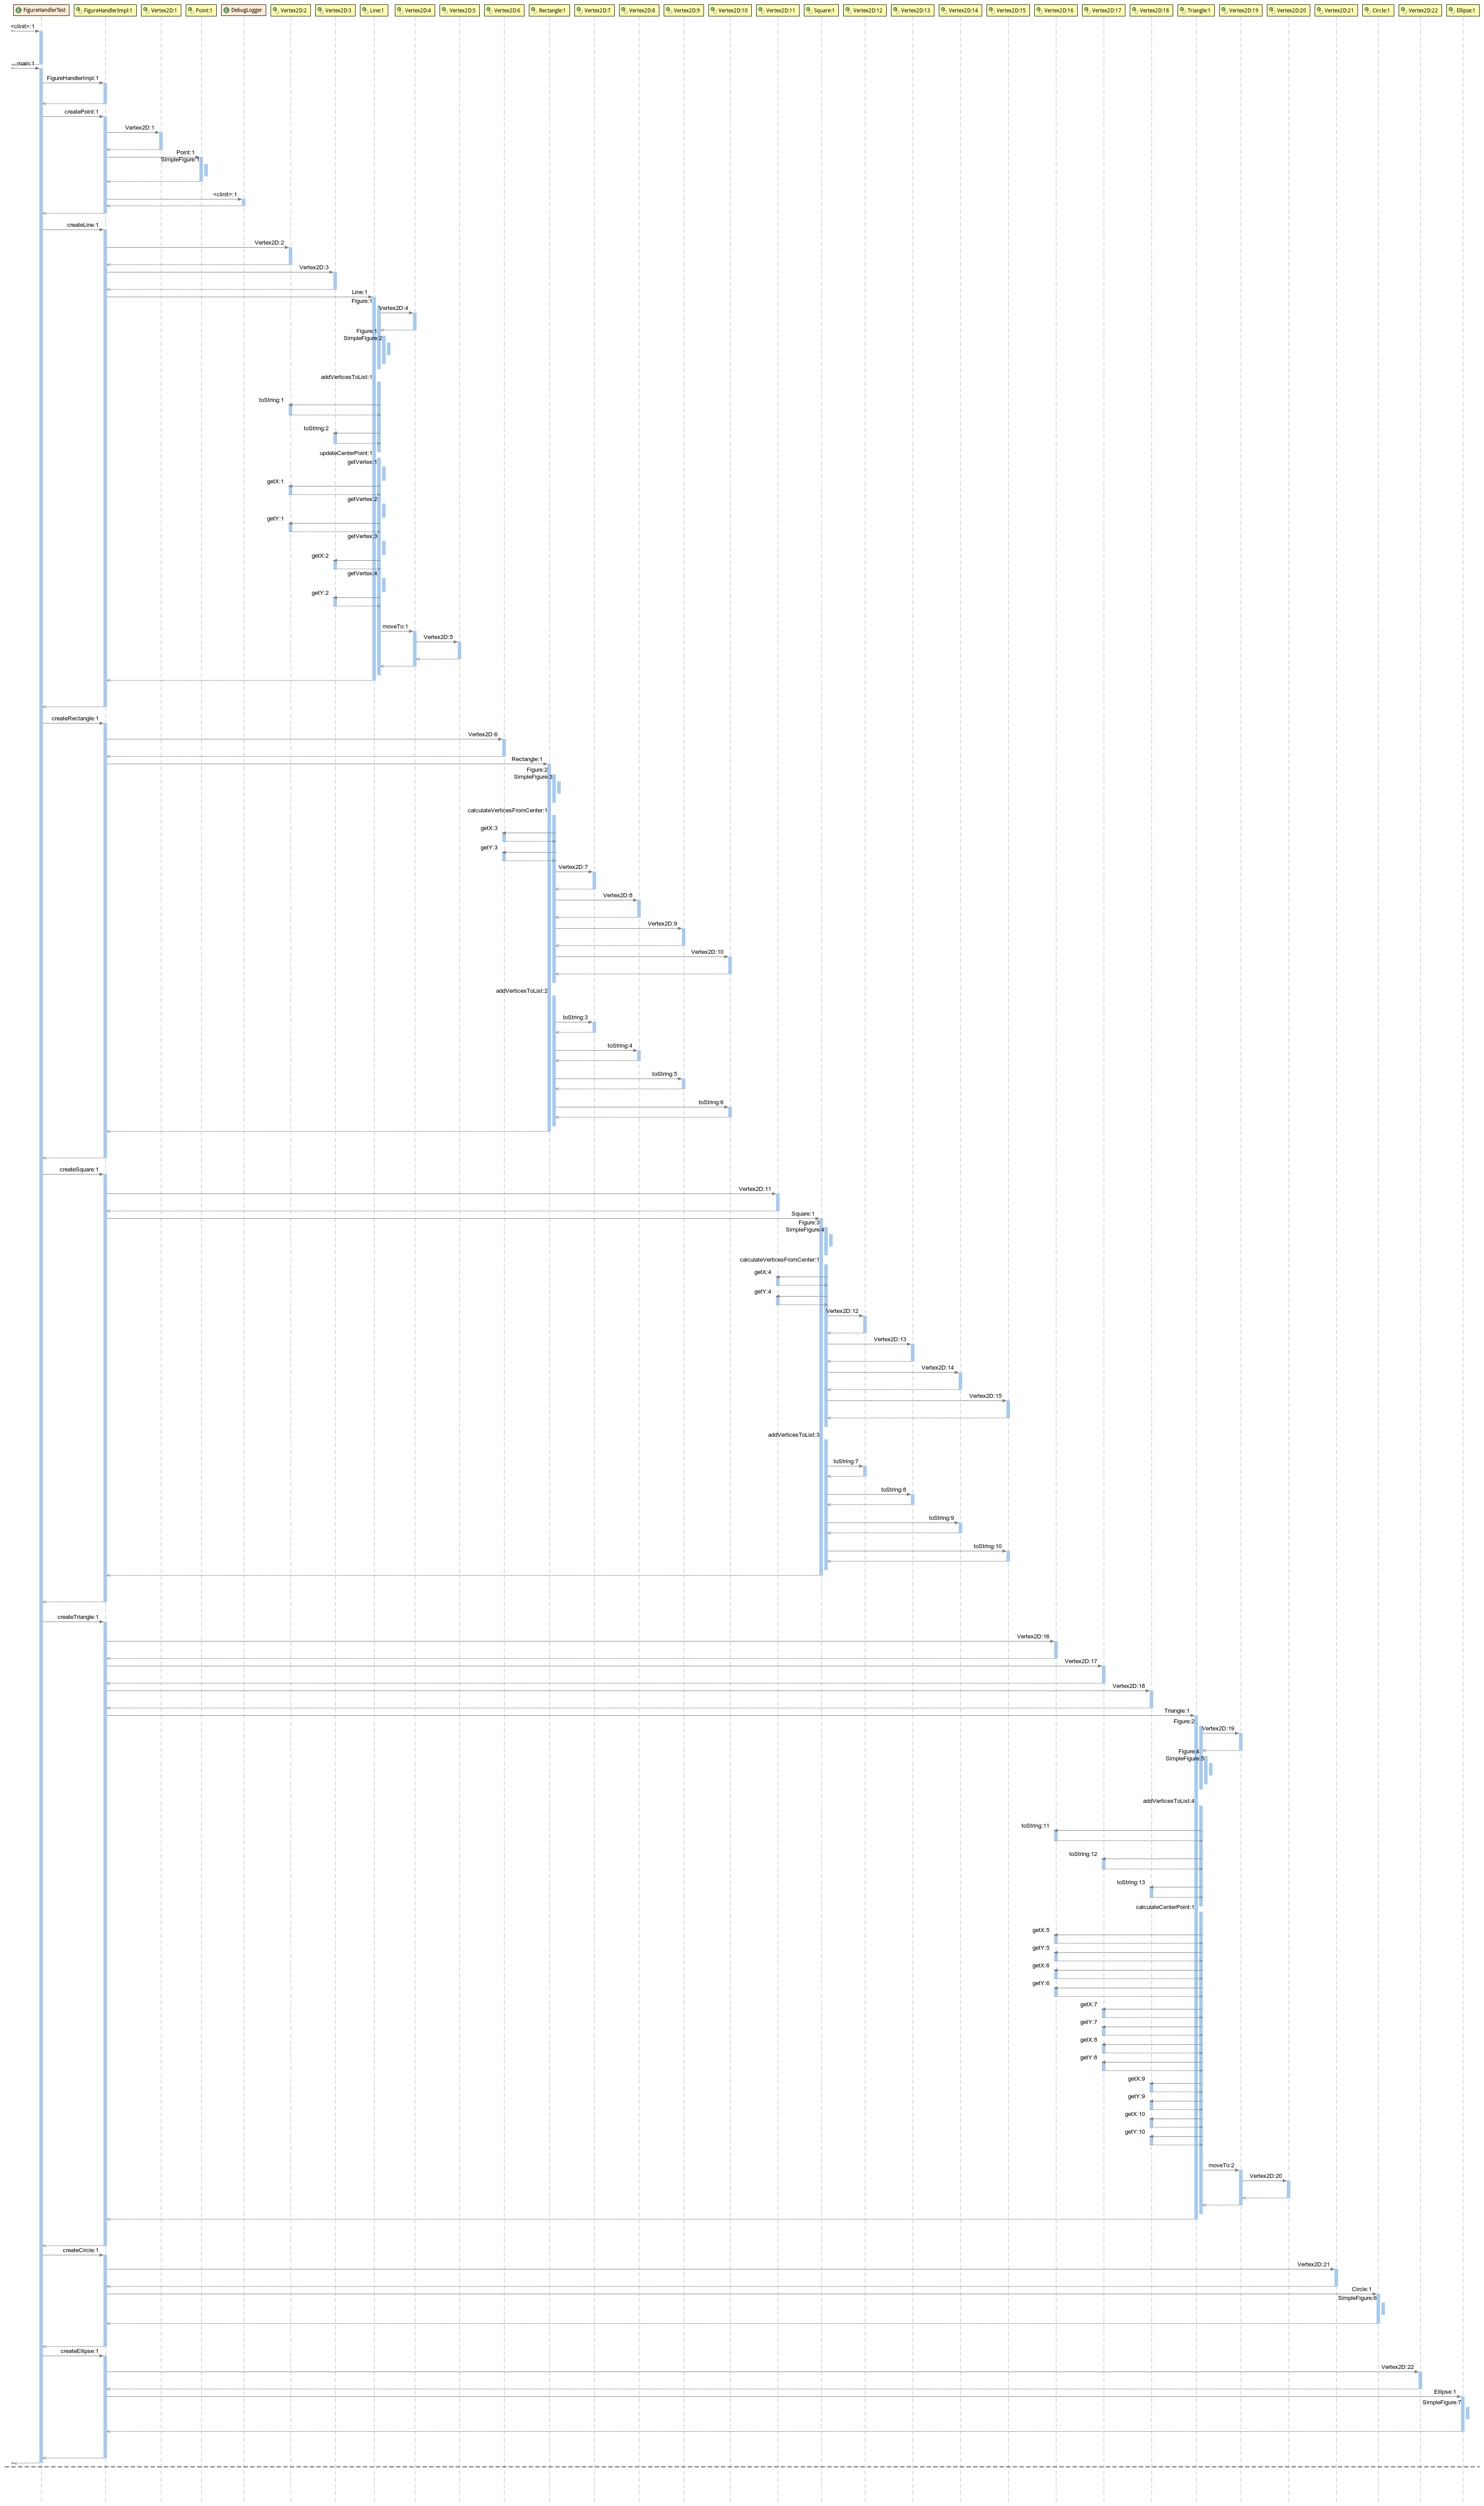
\includegraphics[width=0.9\linewidth]{diagram/figureHandlerTest_All_Sequence-Diagram.png}
\caption{Sekvensdiagram för test av alla figurer. 
%{\tiny(\texttt{diagram/figureHandlerTest\_All\_Sequence-Diagram.png})}
}
\label{fig:sekv-all}
%\end{sidewaysfigure}
\end{figure}

\begin{figure}[ht]
\centering
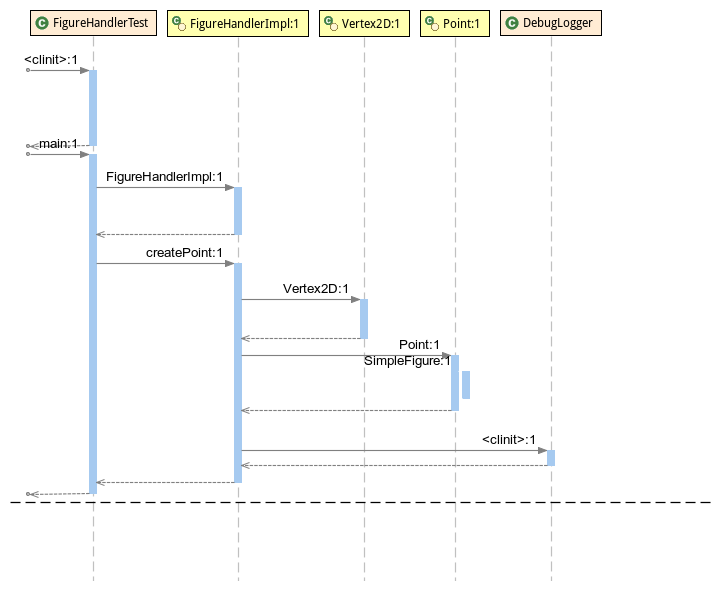
\includegraphics[width=\linewidth]{diagram/figureHandlerTest_Point_Sequence-Diagram.png}
\caption{Sekvensdiagram för \texttt{Point}.
%{\tiny(\texttt{diagram/figureHandlerTest\_Point\_Sequence-Diagram.png})}
}
\label{fig:sekv-point}
\end{figure}

\begin{figure}[ht]
\centering
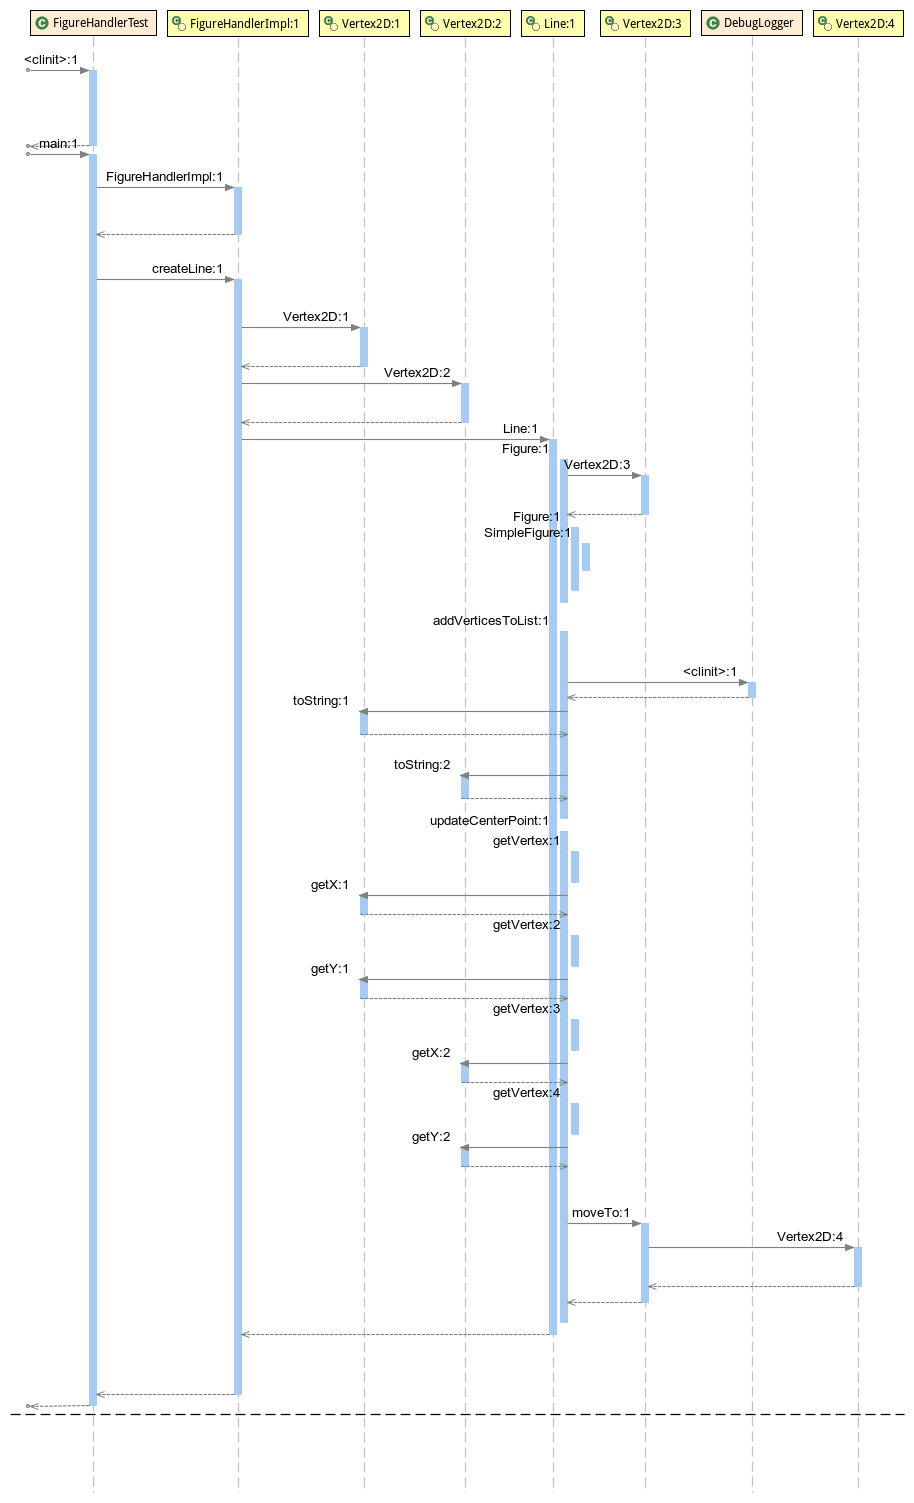
\includegraphics[width=0.8\linewidth]{diagram/figureHandlerTest_Line_Sequence-Diagram.png}
\caption{Sekvensdiagram för \texttt{Line}.
%{\tiny(\texttt{diagram/figureHandlerTest\_Line\_Sequence-Diagram.png})}
}
\label{fig:sekv-line}
\end{figure}

\begin{figure}[ht]
\centering
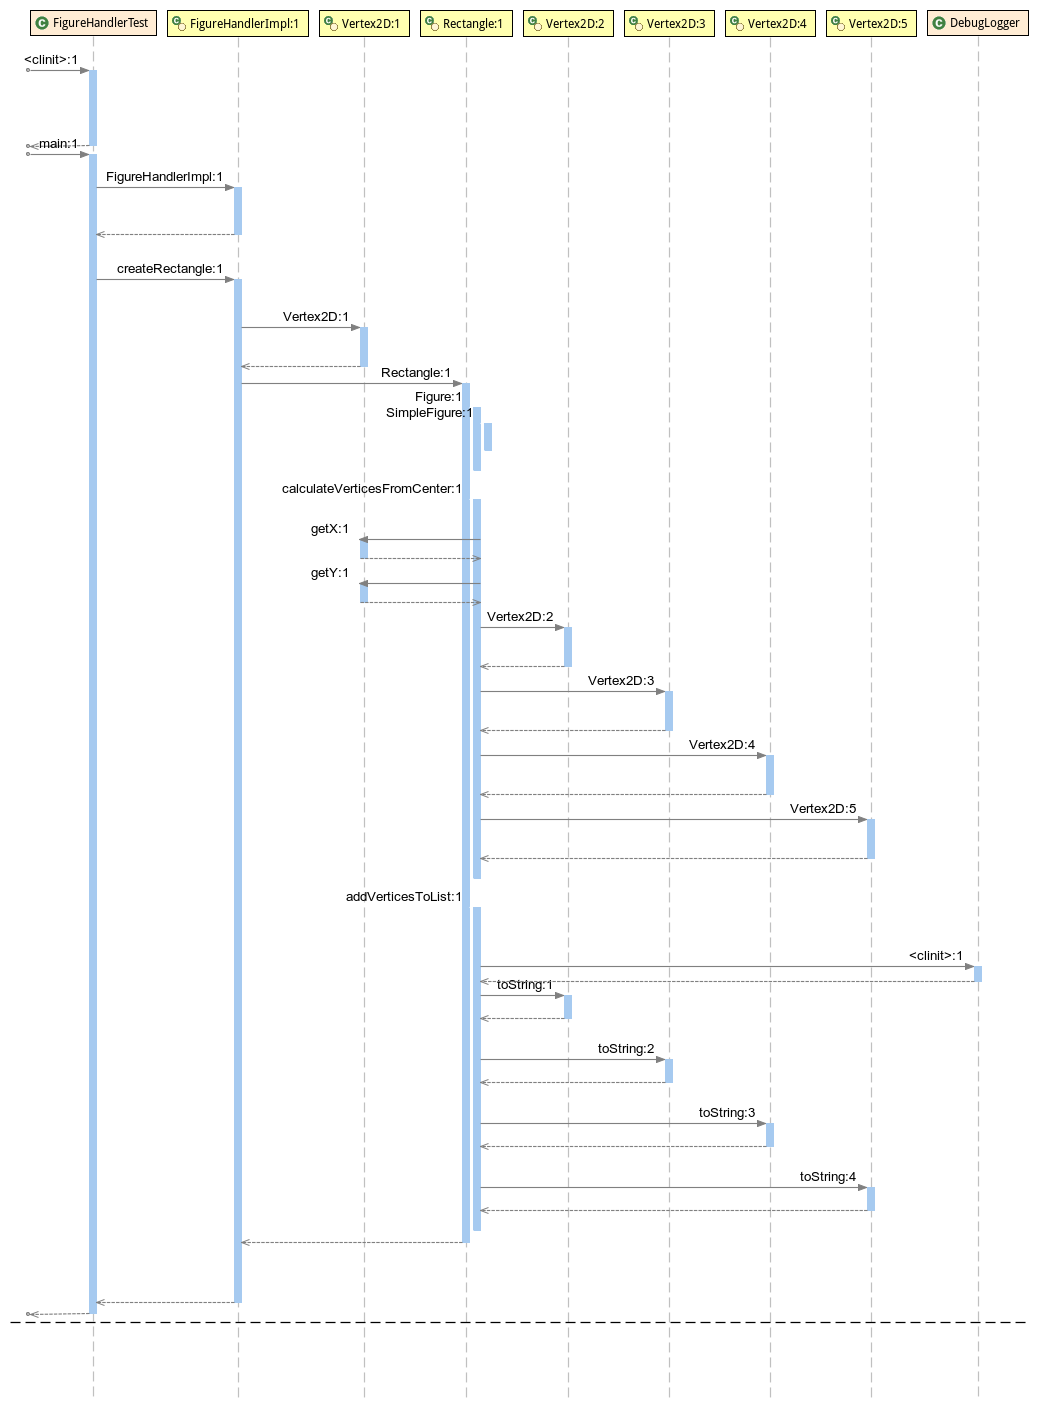
\includegraphics[width=\linewidth]{diagram/figureHandlerTest_Rectangle_Sequence-Diagram.png}
\caption{Sekvensdiagram för \texttt{Rectangle}.
%{\tiny(\texttt{diagram/figureHandlerTest\_Rectangle\_Sequence-Diagram.png})}
}
\label{fig:sekv-rect}
\end{figure}

\begin{sidewaysfigure}
%\begin{figure}[ht]
\centering
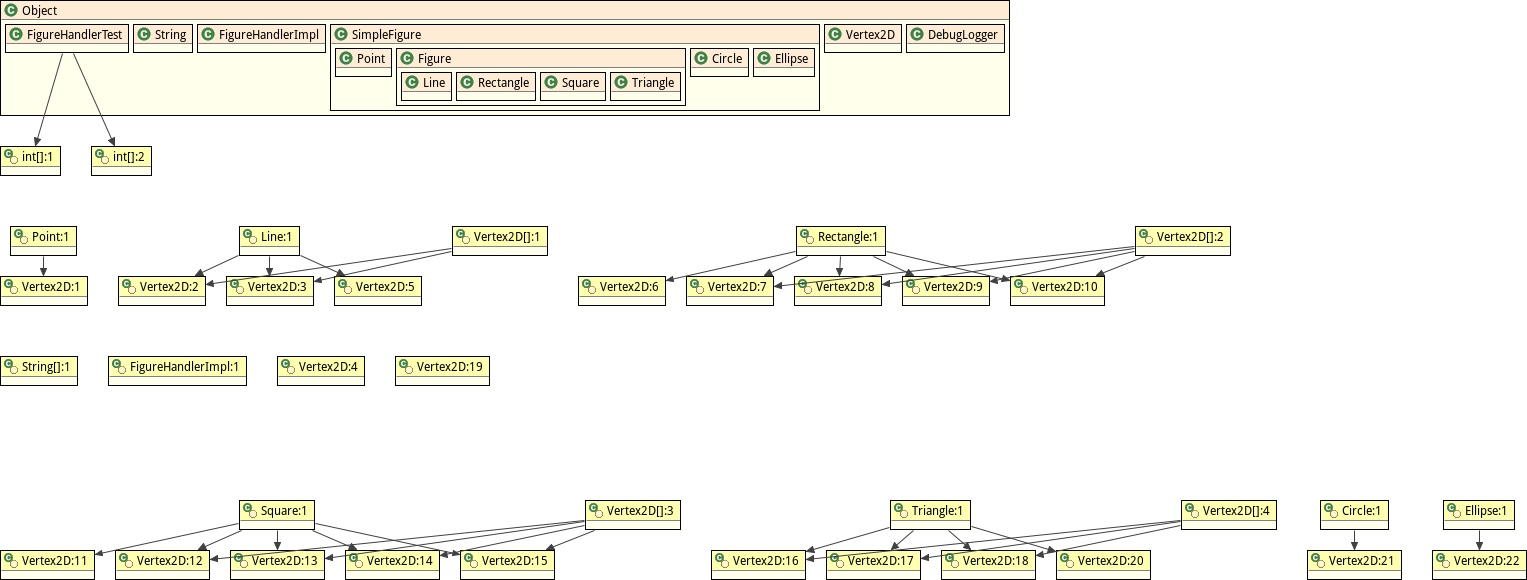
\includegraphics[width=\linewidth]{diagram/figureHandlerTest_All_Object-Diagram.png}
\caption{Objektdiagram för test av alla figurer.
%{\tiny(\texttt{diagram/figureHandlerTest\_All\_Object-Diagram.png})}
}
\label{fig:obj-all}
%\end{figure}
\end{sidewaysfigure}

\begin{figure}[ht]
\centering
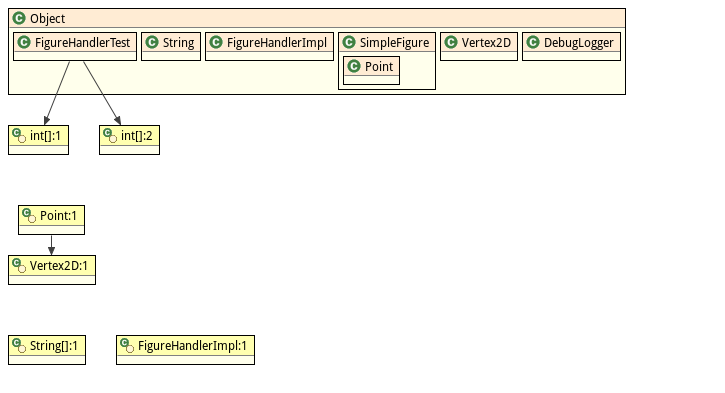
\includegraphics[width=\linewidth]{diagram/figureHandlerTest_Point_Object-Diagram.png}
\caption{Objektdiagram för \texttt{Point}.  
%{\tiny(\texttt{diagram/figureHandlerTest\_Point\_Object-Diagram.png})}
}
\label{fig:obj-point}
\end{figure}

\begin{figure}[ht]
\centering
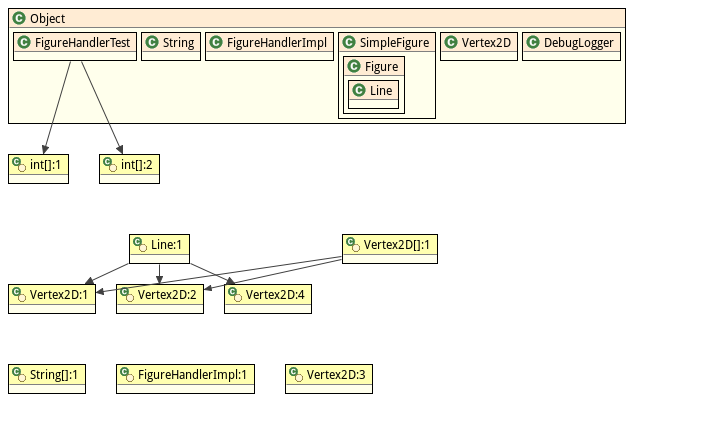
\includegraphics[width=\linewidth]{diagram/figureHandlerTest_Line_Object-Diagram.png}
\caption{Objektdiagram för \texttt{Line}.  
%{\tiny(\texttt{diagram/figureHandlerTest\_Line\_Object-Diagram.png})}
}
\label{fig:obj-line}
\end{figure}

\begin{figure}[ht]
\centering
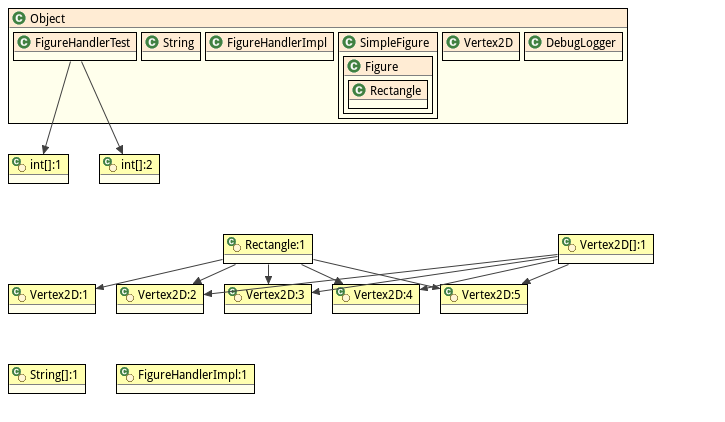
\includegraphics[width=\linewidth]{diagram/figureHandlerTest_Rectangle_Object-Diagram.png}
\caption{Objektdiagram för \texttt{Rectangle}.
%{\tiny(\texttt{diagram/figureHandlerTest\_Rectangle\_Object-Diagram.png})}
}
\label{fig:obj-rect}
\end{figure}

\subsection{}\label{sec:uppg3b}
\subsubsection*{Frågeställning}
Skriv klasserna som implementerar interfacen i styrnings-API:et enligt figur 7.

\subsubsection*{Lösning}
Se bifogad källkod. Lösningen använder \texttt{StringBuilder} för att
konkatenera resultatet från superklassens \texttt{toString}-metod med klassens
egna data.


\subsection{}\label{sec:uppg3c}
\subsubsection*{Frågeställning}
Diskutera: Varför används typer som \texttt{List<FigureType>} i FigureHandler?
Kan man inte använda bara List? Eller en array?


\subsubsection*{Lösning}
Användningen av en \texttt{List} framför en vanlig array motiveras med att en
array inte kan ändra storlek dynamiskt. Storleken definieras vid skapande av
arrayen och är därefter fixerad. En \texttt{List} har flera användbara
funktioner som saknas för arrays. Genom att skriva något i stil med
\texttt{List<Figure>} specifieras vilken typ av objekt listan kan innehålla.
Det fungerar som en slags felkontroll där kompilatorn ger varningar om ett
inkompatibelt objekt stoppas in.


